% tikz
\begin{frame}{TikZ and Plotting}{Introduction}
\small
TikZ is probably the most complex and powerful tool to create graphic elements
in \LaTeX. There are so many options and commands that it is out of the scope of
this session. A small jist of this is shown in the following examples.\\
\vspace{1em}

TikZ uses PGF (Portable Graphics Format) is a macro package for creating
graphics within \LaTeX.

\begin{columns}
    \begin{column}{0.3\textwidth}
        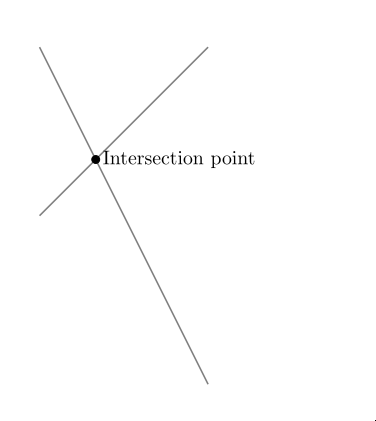
\includegraphics[width=\textwidth]{plotting1.png}
    \end{column}
    \begin{column}{0.7\textwidth}
        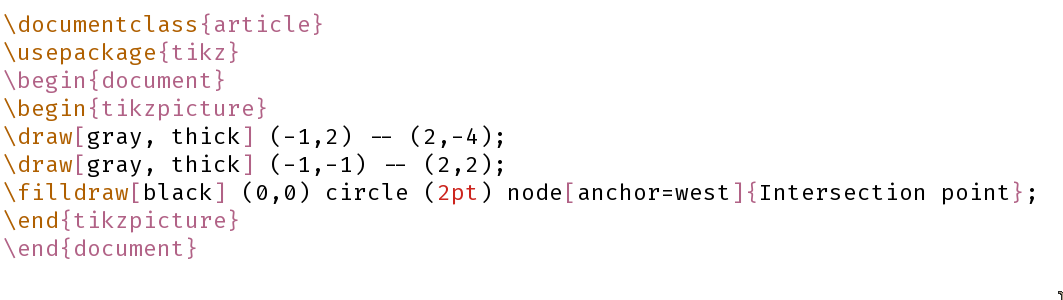
\includegraphics[width=\textwidth]{plotting1_code.png}
    \end{column}
\end{columns}

\end{frame}

\begin{frame}{TikZ and Plotting}{Plotting using TikZ}
\small
When you plot a function, the coordinates of the plot data can be computed by
evaluating a mathematical expression. Since \texttt{pgf} comes with a mathematical
engine, you can specify this expression and then have TikZ produce the desired
coordinates for you, automatically.

\begin{columns}
    \begin{column}{0.4\textwidth}
        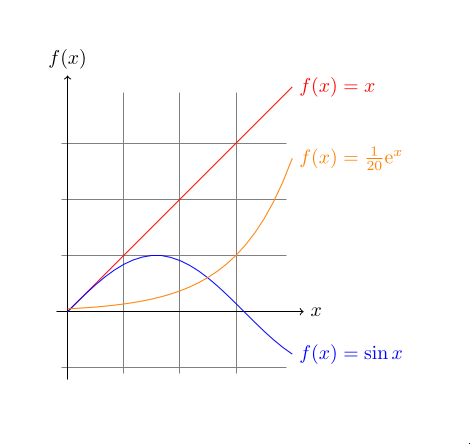
\includegraphics[width=\textwidth]{plotting2.png}
    \end{column}
    \begin{column}{0.6\textwidth}
        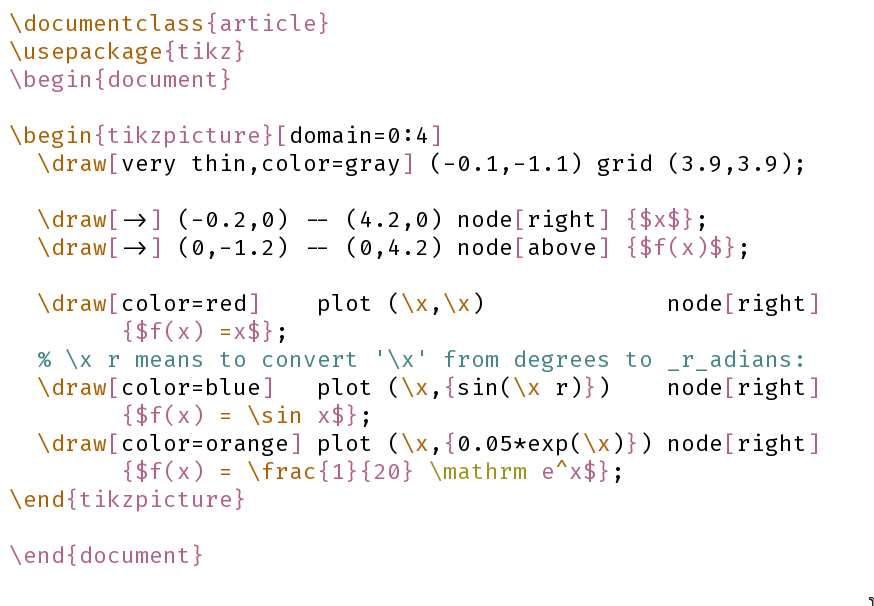
\includegraphics[width=\textwidth]{plotting2_code.png}
    \end{column}
\end{columns}

\end{frame}


\begin{frame}{TikZ and Plotting}{3-rd Party tools and TikZ}

    \tiny
    I have used TikZ in my 'Automata Theory' assignment to make a finite state
    machine. \href{https://www.cs.unc.edu/~otternes/comp455/fsm\_designer/}{This}
    website, is a simple GUI to create Finite State Machines. \vspace{1em}

    Also used the same tool to make a turing machine:
    \center
    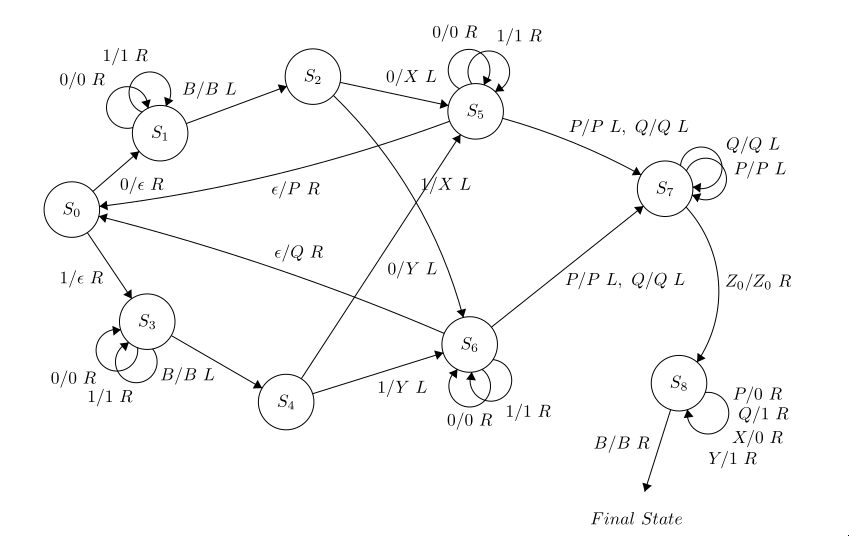
\includegraphics[width=0.7\textwidth]{plotting3.png}

\end{frame}
